\chapter{Сессии}\label{chap:sessions}

HTTP является протоколом без состояния. И хотя некоторые рассматривают это как недостаток, сторонники RESTful веб-разработки восхваляют это как плюс. Ведь когда состояние отсутствует, тогда приложение легче масштабировать, доступно автоматическое кэширование и многие другие приятные побочные эффекты. В общем, вы можете провести много параллелей с неизменяемой природой Haskell.

Насколько это возможно, RESTful приложениям следует избегать сохранения состояния с информацией о взаимодействии с клиентом. Тем не менее, иногда это неизбежно. Классическим примером является такая функциональность, как корзина покупок, но и другие, более обычные взаимодействия, наподобие должной обработки входа в систему, могут быть значительно улучшены путём правильного использования сессий.

В этой главе описывается, как Yesod сохраняет данные сессии, как вы можете получить доступ к этим данным, а также некоторые специальные функции, которые помогут вам использовать сессии наилучшим образом.

\section{Clientsession}

Одним из первых пакетов, которые отделились от Yesod, был \footnotehref{http://hackage.haskell.org/package/clientsession}{clientsession}. Этот пакет использует шифрование и подписи для хранения данных в куки-файлах на стороне клиента. Шифрование препятствует изучению данных пользователем, а подпись гарантирует, что сессия не была ни захвачена, ни изменена.

Возможно, с точки зрения эффективности, хранение данных в куки звучит как плохая идея: ведь это означает, что данные должны быть отправлены на каждый запрос. Однако на практике, clientsession может значительно улучшить производительность.

\begin{itemize}
  \item Для обработки запроса не требуется обращаться к базе данных на стороне сервера.
  \item Легко масштабировать по горизонтали: каждый запрос содержит всю информацию, необходимую для ответа.
  \item Для того чтобы уменьшить нагрузку на канал, сайты могут предоставлять статический контент с отдельного доменного имени, чтобы избежать накладных расходов на передачу куки для каждого запроса.
\end{itemize}

Сохранение мегабайт информации в сессии будет плохой идеей. И поэтому большинство рекомендаций по реализаций сессий не рекомендуют такую практику. Если вам действительно нужно сберегать много данных для пользователя, то лучше хранить ключ поиска в сессии, а фактические данные в базе данных.

Все взаимодействия с clientsession обрабатывается внутри Yesod, но есть несколько мест, где вы можете немного настроить его поведение.

\section{Управление сессией}

В классе типов Yesod существуют три функции, которые управляют работой сессии. Функция \footnotehref{http://hackage.haskell.org/packages/archive/yesod-core/latest/doc/html/Yesod-Core.html\#v:encryptKey}{\lstinline'encryptKey'} возвращает текущий ключ шифрования. По умолчанию она берёт его из локального файла, чтобы сессии могли сохраняться между перезагрузками базы данных. Если этот файл не существует, то он будет автоматически создан и заполнен случайными данными. А если переопределить эту функцию так, чтобы она возвращала \lstinline'Nothing', то сессии будут отключены.

\begin{remark}
Зачем отключать сессии? Они вносят накладные расходы на \textbf{производительность}. При нормальных обстоятельствах, эти расходы минимальны, особенно по сравнению с доступом к базе данных. Однако когда имеешь дело с очень простыми задачами, эти накладные расходы могут стать заметными. Будьте осторожны с отключением сессий: ведь это также отключит такую функциональность, как защиту от подделки межсайтовых запросов (Cross-Site Request Forgery, сокращённо CSRF).
\end{remark}

Следующая функция \footnotehref{http://hackage.haskell.org/packages/archive/yesod-core/latest/doc/html/Yesod-Core.html\#v:clientSessionDuration}{\lstinline'clientSessionDuration'}. Эта функция возвращает количество минут, в течении которых сессия должна быть активной. Значение по умолчанию составляет 120 (2 часа).

Это значение в конечном итоге влияет на куки сессии двумя способами: во-первых, оно определяет срок действия куки. Однако что более важно, время окончания сессии закодировано внутри подписи сессии. Когда Yesod расшифровывает подпись, он проверяет, в прошлом ли дата, и если да, то значения сессии игнорируются.

\begin{remark}
Каждый раз, когда Yesod посылает ответ клиенту, он отправляет куки с обновлённым сроком годности. Таким образом, даже если вы не изменяете сами значения сессии, срок сессии не истечёт, если пользователь просто продолжает просматривать ваш сайт.
\end{remark}

И это подводит к последней функции: \footnotehref{http://hackage.haskell.org/packages/archive/yesod-core/latest/doc/html/Yesod-Core.html\#v:sessionIpAddress}{\lstinline'sessionIpAddress'}. По умолчанию, чтобы предотвратить перехват сессии, Yesod также кодирует в куки IP-адрес клиента. В общем, это хорошая вещь. Тем не менее, некоторые провайдеры держат своих пользователей за прокси серверами, которые переписывают их IP-адреса, иногда меняя исходный адрес в середине сессии. Если это произойдёт, и \lstinline'sessionIpAddress' включён, то сессия пользователя будет сброшена. Установка же этого параметра в \lstinline'False' позволит сессии продолжать в таких условиях ценой подвержения пользователя возможному захвату сессии.

\section{Работа с сессией}

Как и в большинстве фреймворков, сессия в Yesod представляет собой хранилище пар ключ-значение. Базовое API сессии сводится к четырём функциям: \lstinline'lookupSession' получает значение для ключа (если имеется), \lstinline'getSession' возвращает все пары ключ/значение, \lstinline'setSession' задаёт значение для ключа, а \lstinline'deleteSession' очищает значение для ключа.

\lstinputlisting{../hs/09-session-example.hs}

\section{Сообщения}

Одно из использований сессий~--- это сообщения. Они используются, чтобы решить одну из обычных задач в веб-разработке: пользователь выполняет POST запрос, веб-приложение делает изменения, а затем должно \emph{одновременно} перенаправить пользователя на новую страницу и отправить ему сообщение об успехе. (Это известно как Post/Redirect/Get).

Yesod предоставляет пару функций, чтобы сделать эту задачу очень простой: \lstinline'setMessage' сохраняет значение в сессии, а \lstinline'getMessage' одновременно считывает последнее значение в сессии и очищает старое значение, так что оно не будет случайно отображено два раза. 

Рекомендуется вызывать \lstinline'getMessage' в \lstinline'defaultLayout', так любое доступное сообщение покажется пользователю немедленно, без необходимости помнить о добавлении вызова \lstinline'getMessage' в каждом обработчике.

\lstinputlisting{../hs/09-messages.hs}

\begin{figure}[tbh]
  \centering
  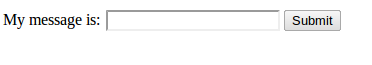
\includegraphics{09-sessions-image-01.png}
  \caption{Первая загрузка страницы, нет сообщения}
\end{figure}

\begin{figure}[tbh]
  \centering
  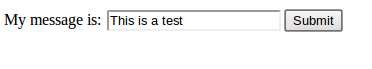
\includegraphics{09-sessions-image-02.png}
  \caption{Новое сообщение введено в текстовое поле}
\end{figure}

\begin{figure}[tbh]
  \centering
  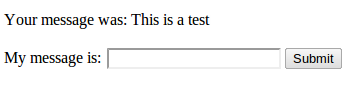
\includegraphics{09-sessions-image-03.png}
  \caption{После отправки формы, сообщение появляется в верхней части страницы}
\end{figure}

\begin{figure}[tbh]
  \centering
  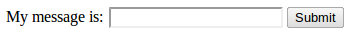
\includegraphics{09-sessions-image-04.png}
  \caption{После обновления, сообщение очищено}
\end{figure}

\section{Пункт назначения}

Не путайте с фильмом ужасов, пункт назначения~--- это понятие которое используется внутри \footnotehref{http://hackage.haskell.org/package/yesod-auth}{yesod-auth}. Предположим, пользователь запрашивает страницу, которая требует аутентификации. Если пользователь ещё не вошёл в систему, вам нужно отправить его на страницу входа. Хорошо продуманное веб-приложение затем \emph{отправит его обратно на первоначально запрошенную страницу}. Это то, что мы называем пунктом назначения. 

Функция \lstinline'redirectUltDest' отправляет пользователя в пункт назначения, установленный в его сессии, очищая это значение в сессии. Так же она берёт значение по умолчанию, в случае, если значение пункта назначения не установлено. Для установки сессии, есть три варианта:

\begin{itemize}
  \item \lstinline'setUltDest' устанавливает пункт назначения в данный URL;
  \item \lstinline'setUltDestCurrent' устанавливает пункт назначения в текущий запрошенный URL;
  \item \lstinline'setUltDestReferer' устанавливает пункт назначения на основе заголовка; \lstinline'Referer' страница, которая привела пользователя на текущую страницу;
\end{itemize}

Давайте рассмотрим небольшой пример приложения. Оно позволит пользователю задать его имя в сессии, а затем скажет ему его имя с другого маршрута. Если имя ещё не было установлено, пользователь будет перенаправлен на страницу ввода имени, с пунктом назначения, установленным в возврат к текущей странице.

\begin{lstlisting}
{-# LANGUAGE OverloadedStrings, TypeFamilies, TemplateHaskell,
             QuasiQuotes, MultiParamTypeClasses #-}

import Yesod

data UltDest = UltDest

mkYesod "UltDest" [parseRoutes|
/ RootR GET
/setname SetNameR GET POST
/sayhello SayHelloR GET
|]

instance Yesod UltDest

instance RenderMessage UltDest FormMessage where
    renderMessage _ _ = defaultFormMessage

getRootR = defaultLayout [whamlet|
<p>
    <a href=@{SetNameR}>Set your name
<p>
    <a href=@{SayHelloR}>Say hello
|]

-- Отобразить форму для ввода имени
getSetNameR = defaultLayout [whamlet|
<form method=post>
    My name is #
    <input type=text name=name>
    . #
    <input type=submit value="Set name">
|]

-- Достать указанное пользователем имя
postSetNameR :: Handler ()
postSetNameR = do
    -- Получить указанное имя и установить его для сессии
    name <- runInputPost $ ireq textField "name"
    setSession "name" name

    -- После того как мы получили имя, перенаправить в пункт назначения.
    -- Если пункт назначения не задан, по умолчанию направляем на домашнюю страницу
    redirectUltDest RootR

getSayHelloR = do
    -- Ищем значение имени установленное в сессии
    mname <- lookupSession "name"
    case mname of
        Nothing -> do
            -- Имя не задано, устанавливаем текущюю станицу как
            -- пункт назначения и перенаправляем на
            -- страницу задания имени - SetName 
            setUltDestCurrent
            setMessage "Please tell me your name"
            redirect SetNameR
        Just name -> defaultLayout [whamlet|
<p>Welcome #{name}
|]

main :: IO ()
main = warpDebug 3000 UltDest
\end{lstlisting}%$

\section{Выводы}

Сессии~--- это способ номер один для преодоления отсутствия состояния в HTTP. Но мы не должны использовать этот чёрный ход всякий раз, когда хотим: отсутствие состояний в веб-приложениях~--- это хорошее свойство, и мы должны уважать его, когда это возможно. Тем не менее, есть определённые случаи, когда важно сохранять некоторое состояние. 

В Yesod очень простой API для работы с сессиями. Он предоставляет хранилише пар ключ-значение, и несколько удобных функций для работы с ними для типичных сценариев использования. При правильном использовании, с небольшой нагрузкой, сессии должны быть скромной частью вашей веб-разработки. 
